\documentclass[a4paper]{article}

% --- Page layout and spacing ---
\usepackage[top=2.5cm, left=3cm, right=3cm, bottom=3cm]{geometry}
\usepackage[utf8]{inputenc}      % input encoding
\usepackage[T1]{fontenc}         % font encoding
\usepackage[english]{babel}
\usepackage{setspace}
\setlength{\parindent}{0pt}      % paragraph indentation
\setlength{\parskip}{0.8em}      % space between paragraphs
\setstretch{1.2}                 % line spacing
\emergencystretch=2em            % reduce overfull \hbox warnings
\usepackage{tocloft}             % section spacing in ToC
\setlength{\cftbeforesecskip}{10pt}
\setlength{\cftbeforesubsecskip}{4pt}
\usepackage{titlesec}            % section title spacing
\titlespacing*{\section}{0pt}{5.0ex plus 1ex minus .2ex}{1.0ex plus .2ex}
\titlespacing*{\subsection}{0pt}{3.0ex plus .5ex minus .2ex}{0.8ex plus .2ex}
\titlespacing*{\subsubsection}{0pt}{2.0ex plus .5ex minus .2ex}{0.8ex plus .2ex}
\usepackage{booktabs}

% --- Math and symbols ---
\usepackage{amsmath, amssymb}    % standard math
\usepackage{empheq}              % boxed equations etc.
\DeclareMathOperator{\artanh}{artanh}
\DeclareMathOperator{\sgn}{sgn}
\usepackage{bm}                  % bold math symbols
\usepackage{cancel}              % strikeout in math
\usepackage{siunitx}             % proper units
\DeclareSIUnit\angstrom{\text{Å}}
\renewcommand{\arraystretch}{0.9}

% --- Graphics and floats ---
\usepackage{graphicx}
\usepackage{float}
\usepackage{wrapfig}
\usepackage[justification=centering]{caption}
\usepackage{subcaption}
\captionsetup[figure]{font=small}

% --- Layout helpers ---
\usepackage{boxedminipage}
\usepackage{enumitem}
\usepackage{afterpage}
\usepackage{changepage}
\usepackage{pdfpages}           % include external PDFs
\usepackage{esvect}             % nice vector arrows
\usepackage{hyperref}           % hyperlinks

% --- Bibliography setup ---
\usepackage{csquotes}
\usepackage[backend=biber,style=numeric,sorting=none]{biblatex}
\addbibresource{references.bib}

% --- Fonts ---
\usepackage{lmodern}            % Computer Modern look across TeX distros

\begin{document}

% ------------------
% --- Title page ---
% ------------------
\begin{titlepage}
  \thispagestyle{empty}
  \begin{center}

    % Title
    \vspace*{1cm}
    {\LARGE \textbf{Rayleigh Scattering}}\\[1.2cm]

    % Subtitle
    {\large Evaluation Report}\\[2cm]

    % Authors
    \large
    \textbf{Cem Boyaci}\\[-1mm]
    {cemb93@zedat.fu-berlin.de}\\[1cm]

    \textbf{Javier Bellido Roldán}\\[-1mm]
    {bellidoroj98@zedat.fu-berlin.de}\\[1cm]

    \textbf{Leon Goldammer}\\[-1mm]
    {lg4278fu@zedat.fu-berlin.de}\\[6cm]

    % Tutor
    \normalsize
    {Tutor: Kenichi Ataka}\\[1.2cm]

    % Footer block
    \textbf{Fortgeschrittenenpraktikum, WS 2025/2026}\\
    Berlin, 09.03.2026\\
    Freie Universität Berlin\\
    Fachbereich Physik

  \end{center}
\end{titlepage}

% -------------------------
% --- Table of contents ---
% -------------------------
\clearpage
\renewcommand*\contentsname{\huge Contents}
{
  \pagenumbering{gobble}
  \tableofcontents
  \clearpage
}
\pagenumbering{arabic}

% --------------------
% --- Introduction ---
% --------------------
\newpage
\setcounter{page}{1}
\section{Introduction}
\label{sec:introduction}

Rayleigh scattering is the elastic scattering of light by particles that are much smaller than the wavelength.
In everyday life it is most famously responsible for the blue appearance of the sky, since short-wavelength light is scattered more efficiently than long-wavelength light~\cite{RAYAnleitung}.

In this experiment, Rayleigh scattering is studied quantitatively in air as a very small but well-defined optical loss process.
The aim is to determine the molecular scattering coefficient $\beta(\lambda)$ of air at a fixed wavelength and to compare the result with the theoretical expectation~\cite{RAYAnleitung}.

A key experimental challenge is that the Rayleigh loss over ordinary laboratory distances is extremely small.
This makes simple transmission measurements impractical, because the signal change would be comparable to typical fluctuations and systematic effects.
The experiment therefore uses an optical arrangement that realizes very large effective path lengths within a compact setup, so that the weak scattering loss becomes measurable in a robust way~\cite{RAYAnleitung}.

% --------------
% --- Theory ---
% --------------
\section{Theory}

\subsection{Rayleigh Scattering}
\label{sec:theory_rayleigh}

Whether light scattering is described as Rayleigh or Mie scattering is mainly determined by how large the scatterers are compared to the wavelength.
This comparison is captured by the size parameter $x$, defined as
\[
x=\frac{2\pi a}{\lambda},
\]

where $a$ is the particle diameter and $\lambda$ is the optical wavelength~\cite{RAYAnleitung}.
For $x\ll 1$ the Mie theory reduces to the Rayleigh regime, which is the relevant case for scattering on atmospheric molecules in air.
In contrast, micrometer-sized particles such as water droplets are not in the molecular Rayleigh limit and instead scatter light in the Mie regime~\cite{RAYAnleitung}.
This is why clouds, which consist of many water droplets, appear white rather than blue.

In the Rayleigh regime, the incident light field makes the electrons in a molecule oscillate, so the molecule behaves like a tiny driven dipole that reemits light~\cite{RAYAnleitung, Miles2001}.
A simple and intuitive picture is to think of the light beam as many photons traveling forward, where occasionally a photon is scattered by a molecule and then continues in a different direction.
The photon energy stays essentially the same in Rayleigh scattering, so the wavelength does not change.
The beam still loses intensity, because intensity measures how much power remains in the original forward direction, and every scattering event redirects a small fraction of that power into other directions.
This is the same mechanism that makes the sky appear blue: shorter wavelengths are scattered more efficiently and are therefore redistributed more strongly into the atmosphere, while the directly transmitted sunlight becomes slightly depleted in blue, shifting its apparent color toward yellow~\cite{RAYAnleitung}.

Quantitatively, the scattered power of a single scatterer is proportional to the incident intensity, and the proportionality constant is the scattering cross section $\sigma(\lambda)$.
In a gas containing many scatterers, it is convenient to use the scattering coefficient $\beta(\lambda)$ (unit $\si{m^{-1}}$), defined by
\begin{equation}
\beta(\lambda)=N\,\sigma(\lambda),
\label{eq:beta_def}
\end{equation}

where $N$ is the number concentration of scatterers~\cite{RAYAnleitung}.
The scattering coefficient $\beta(\lambda)$ has the unit of an inverse length and quantifies how strongly a beam is attenuated by Rayleigh scattering per unit distance.
For a homogeneous gas, the transmitted intensity follows the Beer--Lambert law,
\[
I(z)=I_0\,e^{-\beta(\lambda)\,z},
\]
where $I_0$ is the intensity at $z=0$.
For short path lengths with $\beta(\lambda)\,z\ll 1$, the exponential can be approximated as $I(z)\approx I_0\left(1-\beta(\lambda)\,z\right)$, which shows that $\beta(\lambda)$ is the fractional loss of forward intensity per unit length.

Rayleigh scattering is characterized by a strong wavelength dependence, with the scattering strength increasing rapidly toward shorter wavelengths.
For molecular Rayleigh scattering, the scattering coefficient can be expressed in terms of the refractive index $n$ of the gas as
\begin{equation}
\beta(\lambda)=\frac{8\pi^{3}}{3N\lambda^{4}}\left(n^{2}-1\right)^{2}.
\label{eq:beta_rayleigh}
\end{equation}

The characteristic $\lambda^{-4}$ scaling is the key result: for a fixed gas composition and density, changing the wavelength has a much stronger effect on $\beta$ than most other parameters~\cite{RAYAnleitung}.

For the experiment, the goal is to determine the molecular scattering coefficient $\beta(\lambda)$ of air and to compare it with the theoretical value from Eq.~\eqref{eq:beta_rayleigh}.
Since typical molecular scattering coefficients in gases are extremely small, the corresponding intensity reduction over ordinary laboratory distances is tiny.
This makes a direct transmission measurement impractical and motivates the use of an optical method that realizes very large effective path lengths within a compact setup~\cite{RAYAnleitung}.

\subsection{Cavity Ring-Down Spectroscopy}
\label{sec:theory_crds}

Cavity ring-down spectroscopy (CRDS) is a time-domain method for measuring extremely small optical losses by storing light in a high-finesse optical cavity and observing its decay.
The cavity consists of two highly reflective mirrors that support a stable optical mode, so that injected light performs many round trips and the effective propagation distance becomes very large compared to the physical cavity length.
Instead of measuring an absolute transmission, CRDS measures a decay constant~\cite{RAYAnleitung, Berden2000}.

In a typical CRDS measurement, the cavity is excited by a short laser pulse that is turned off rapidly compared to the subsequent decay.
After the excitation ends, light remains trapped in the cavity mode and a small fraction is transmitted through one of the mirrors during each round trip.
This transmitted fraction is detected as a function of time, and the measured signal follows an exponential decay
\begin{equation}
I(t)=I_0\,e^{-t/\tau},
\label{eq:crds_decay}
\end{equation}

where $I_0$ is the intensity at the beginning of the decay and $\tau$ is the ring-down time~\cite{RAYAnleitung}.
A useful way to interpret this exponential decay is to compare it with Beer--Lambert attenuation: there the intensity decreases exponentially with propagation distance, whereas here it decreases exponentially with time because the circulating light covers an increasing path length $z\approx ct$ as time passes.
The ring-down time is the characteristic time scale on which the intracavity intensity drops by a factor $e$, so it quantifies the total fractional loss per unit time experienced by the stored light.

\begin{figure}[H]
  \centering
  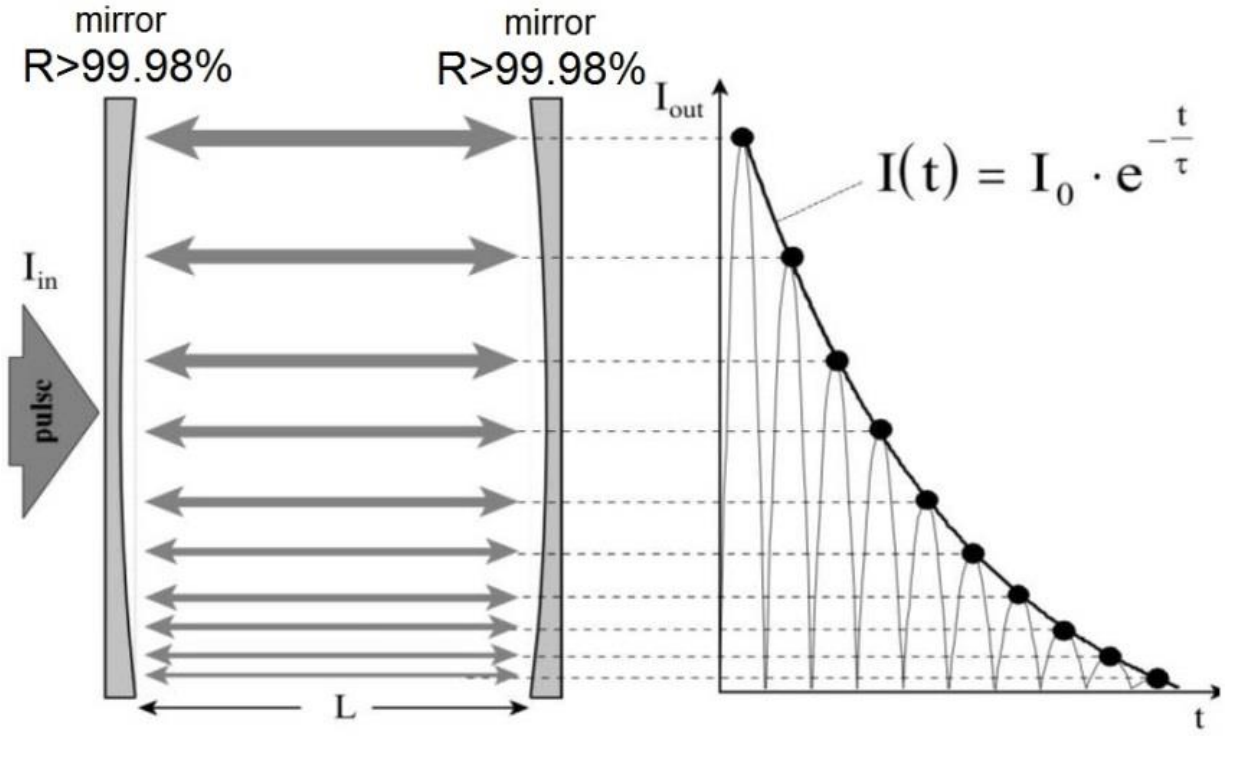
\includegraphics[width=0.9\linewidth]{../resources/figures/crds_principle.png}
  \caption{Principle of a CRDS measurement.
  A short laser pulse is injected into a two-mirror cavity with reflectivity $R>99.98\%$ and the transmitted intensity decays exponentially as $I(t)=I_0 e^{-t/\tau}$~\cite{RAYAnleitung}.}
  \label{fig:crds_principle}
\end{figure}

To connect $\tau$ with cavity losses, consider first an evacuated cavity where losses inside the cavity volume are negligible.
In that case the dominant loss is the finite mirror reflectivity, so the intensity is reduced by approximately the same fraction during each round trip.
For mirror reflectivity $R(\lambda)\approx 0.9998$, one obtains the standard relation
\[
\tau_0(\lambda)=\frac{L}{c\left(1-R(\lambda)\right)},
\]
where $L$ is the cavity length and $c$ is the speed of light~\cite{RAYAnleitung}.
The quantity $\tau_0$ therefore represents the baseline decay time of the empty cavity and is set mainly by the mirror reflectivity, while additional losses such as imperfect alignment or geometrical escape can shorten it further.

If a gas is present in the cavity, photons can be removed from the cavity mode by scattering and absorption inside the cavity volume.
Such loss processes can be described by an extinction coefficient per unit length, which for this experiment is dominated by the scattering coefficient $\beta(\lambda)$ introduced in Eq.~\eqref{eq:beta_def}.
The additional loss shortens the ring-down time from $\tau_0$ to a smaller value $\tau$.
A particularly useful feature of CRDS is that the mirror contribution can be eliminated by comparing measurements with and without the additional loss mechanism.
One finds
\begin{equation}
\beta(\lambda)=\frac{1}{c}\left(\frac{1}{\tau(\lambda)}-\frac{1}{\tau_0(\lambda)}\right).
\label{eq:beta_from_taus}
\end{equation}

Equation~\eqref{eq:beta_from_taus} is the central working equation of the experiment, because it allows the weak molecular scattering loss to be extracted from a difference of decay rates without requiring knowledge of the absolute mirror reflectivity~\cite{RAYAnleitung}.
The role of CRDS in this experiment is therefore to realize an effectively very long optical path length and to transform the tiny Rayleigh loss into a measurable change of the ring-down time.

% --------------------------
% --- Experimental Setup ---
% --------------------------
\section{Experimental Setup}
\label{sec:exp_setup}

A schematic overview of the CRDS measurement setup is shown in Fig.~\ref{fig:crds_setup}.
The experiment combines a pulsed laser source, a high-finesse optical cavity, a time-resolved detection chain, and a vacuum and gas-handling system to alternate between an evacuated reference measurement and an air-filled measurement.
All optical components are mounted on an optical rail that is screwed onto a standard wooden laboratory table (i.e.\ no vibration-isolated optical table is used).

\vspace{1em}
\begin{figure}[H]
  \centering
  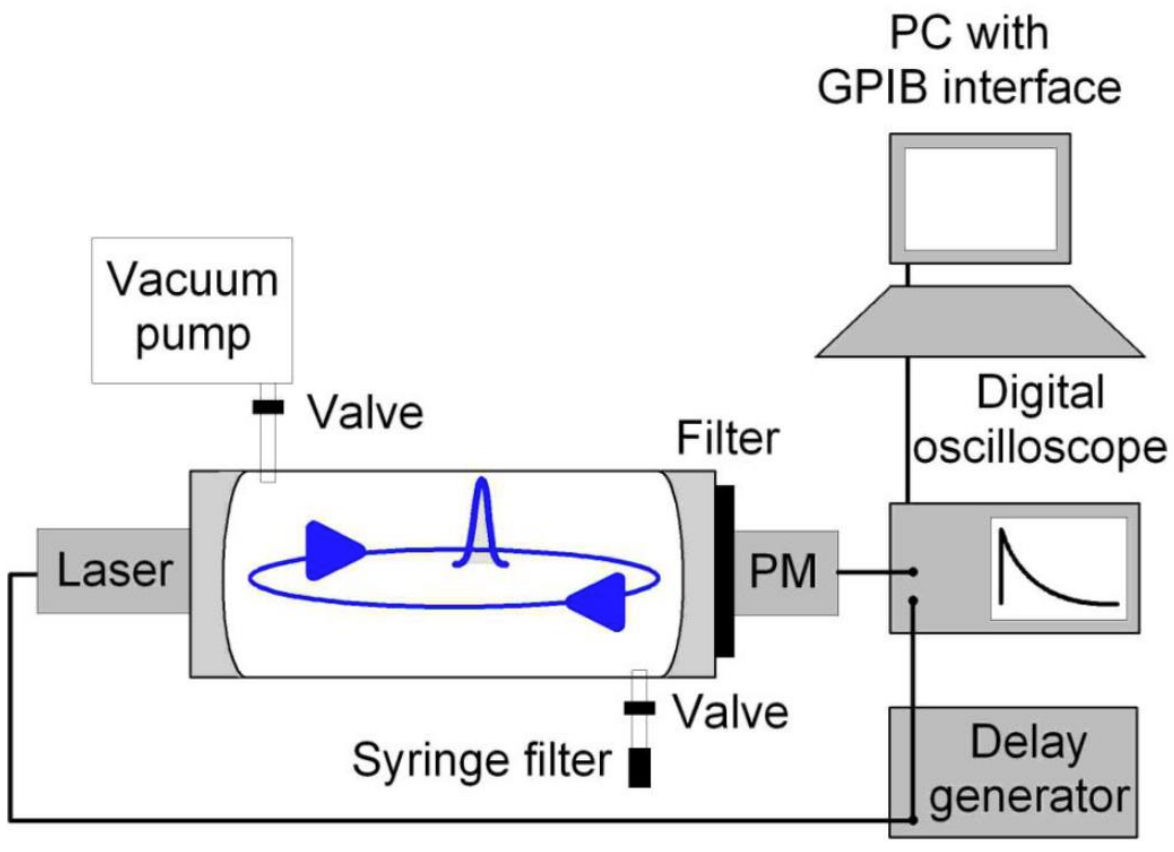
\includegraphics[width=0.97\linewidth]{../resources/figures/crds_setup.png}
  \caption{CRDS measurement setup as used in the experiment.
  The pulsed laser injects light into the optical cavity, the transmitted leakage light is detected with a photomultiplier (PM) after an optical filter and recorded on a digital oscilloscope, and the cavity can be evacuated or filled with filtered ambient air using valves, a vacuum pump, and a syringe filter~\cite{RAYAnleitung}.}
  \label{fig:crds_setup}
\end{figure}

The optical cavity consists of two highly reflective spherical mirrors arranged as a stable resonator with a fixed mirror separation L=\SI{50}{cm} and mirror radius of curvature r=\SI{100}{cm}.
The mirrors have a reflectivity of $R>99.98\%$, so only a very small fraction of the intracavity light is transmitted through the mirror coatings during each round trip.
A short laser pulse from the pulsed laser diode head (PicoQuant LDH-D-C-405, wavelength \SI{405}{nm}, pulse power up to \SI{100}{mW}, repetition rate up to \SI{100}{Hz}) is injected into the cavity through the input mirror, and after the excitation ends the remaining intracavity light decays due to the total losses of the resonator~\cite{RAYAnleitung}.
Between the laser diode head and the cavity entrance, two pinhole apertures are positioned along the beam path over a distance of roughly \SI{50}{cm}.
These apertures define the nominal optical axis and serve as a practical alignment aid: the laser beam is adjusted to pass centrally through both pinholes before entering the cavity, which helps to ensure near-collinear injection and reduces angular misalignment during the subsequent cavity optimization.

For the adjustment of the optical axis and cavity alignment, an additional continuous-wave green laser (wavelength \SI{532}{nm}) is used.
Since this wavelength lies outside the high-reflectivity range of the cavity mirrors, the green beam is transmitted well and provides a clearly visible aid for coarse alignment before optimizing the ring-down signal at \SI{405}{nm}~\cite{RAYAnleitung}.

The light transmitted through the output mirror forms a beam that is measured with a photomultiplier (Hamamatsu H7826) placed behind the cavity.
An optical band-pass filter is positioned in front of the detector to suppress background light and improve the signal-to-noise ratio at the laser wavelength.
The detector output is recorded on a digital oscilloscope (Rohde \& Schwarz HMO1522), which is triggered by the delay generator (Stanford DG545) that also controls the laser pulse timing, ensuring a reproducible time reference for each ring-down trace.
The recorded decay curves are then used to extract the ring-down times $\tau_0$ and $\tau$ by fitting Eq.~\eqref{eq:crds_decay}.
Data can be stored on the oscilloscope and transferred to a PC via a GPIB interface for further analysis~\cite{RAYAnleitung}.

To separate mirror losses from molecular scattering losses, the cavity is operated under two different gas conditions.
First, the cavity is evacuated using a vacuum pump while the pressure is monitored by a manometer, yielding the reference ring-down time $\tau_0$ that is dominated by mirror and alignment losses.
The manometer measures the pressure difference between the cavity and the ambient atmosphere, so a reading of \SI{0}{mbar} corresponds to air at atmospheric pressure, while evacuation leads to negative readings.
Second, the cavity is filled with ambient air at atmospheric pressure to obtain $\tau$, where the additional loss is dominated by Rayleigh scattering in the gas volume.
To reduce unwanted contributions from aerosols, incoming air is passed through a syringe filter with pore diameter \SI{2}{\micro\meter} before entering the cavity, so that the measured additional loss is attributed as closely as possible to molecular scattering~\cite{RAYAnleitung}.
Ambient pressure is measured with a precision barometer (Greisinger GPB 3300) and the ambient temperature is read from an analog glass thermometer (model not specified).

% -----------------
% --- Procedure ---
% -----------------
\section{Procedure}
\label{sec:procedure}

The measurement consists of an alignment phase and a data acquisition phase.
Alignment is performed first with the continuous-wave green laser at \SI{532}{nm} and is then refined with the pulsed laser at \SI{405}{nm} while monitoring the ring-down signal on the oscilloscope.

\subsection{Alignment}

\paragraph{Coarse alignment with the green laser:}
At the beginning, the cavity alignment is typically not optimized and the transmitted beam does not reliably pass through the cavity.
The green alignment laser is switched on because the cavity mirrors transmit \SI{532}{nm} light well, so the beam path through the cavity is directly visible.

First, the green beam is adjusted to propagate straight along the nominal optical axis defined by the pinholes.
The laser head position is tuned so that the beam passes centrally through the first two pinholes, which are kept nearly closed to make the beam spot position clearly visible.
In addition, backreflections from the pinholes and from the laser diode head are used as an alignment check: the alignment is considered good when the reflected spot lands on or very near the point where the beam exits the diode.
The goal is that the beam also hits the third pinhole (the cavity entrance) centrally.

Next, the cavity mirrors are aligned using the four adjustment screws.
The mirror tilts are varied until the green beam exits the cavity at the downstream end.
A sheet of paper is held in front of the cavity exit to observe the transmitted spot and to ensure that the exiting beam is centered so that it later hits the photomultiplier input centrally.

\paragraph{Switch to the blue laser and pre-alignment:}
After the coarse alignment is achieved, the green laser is replaced by the pulsed \SI{405}{nm} laser diode.
The laser output power is set to a moderate value of about \SI{40}{mW} to obtain a stable signal while avoiding excessive heating of the diode head.
The pulse length is set to \SI{100}{\micro\second} and the repetition frequency to \SI{5}{Hz}, so that the cavity is excited by well-separated pulses and each ring-down event can be recorded without overlap.
The \SI{405}{nm} beam position is then adjusted so that it passes through the first two pinholes and hits the cavity entrance pinhole as centrally as possible.
This step is more difficult than with the green laser because the \SI{405}{nm} beam spot is less visible to the eye, so the pinholes are again kept nearly closed and backreflections are used as an additional indicator of a well-centered beam.

Although the mirror alignment from the green laser provides a good starting point, it remains a coarse alignment.
Therefore, small additional adjustments of the mirror screws are typically still required after switching to \SI{405}{nm}, even if the blue beam is well centered on the cavity entrance.

\paragraph{Signal optimization on the oscilloscope:}
The photomultiplier detector is mounted at the cavity output and connected to its power supply and to the oscilloscope input.
The delay generator is used to trigger the oscilloscope and the laser pulse timing so that the ring-down trace is displayed reproducibly.

To find and maximize the ring-down signal, the mirror screws are adjusted while continuously observing the oscilloscope trace.
The detector gain is kept as low as possible to avoid saturation and is only increased when no signal above the noise floor is visible.
Once a ring-down trace emerges from the noise, each of the four mirror screws is adjusted sequentially to maximize the observed signal amplitude and to obtain a clean exponential decay with minimal noise.
After one optimization cycle over all four screws, the detector gain is reduced again (if possible) and the optimization cycle is repeated to further improve signal quality.

\subsection{Data acquisition}
Data acquisition starts from an aligned cavity under vacuum.
The LabVIEW program is started to record the oscilloscope trace and save it as a \texttt{.csv} file.
The oscilloscope time axis is set such that the laser pulse onset defines $t=0$, while negative times correspond to the pre-trigger region.

Each recorded trace is opened in the provided fitting software to obtain an immediate estimate of the ring-down time $\tau$ from an exponential fit.
This quick fit is used as an consistency check to ensure that the measured values are plausible and that the vacuum ring-down time satisfies $\tau_0>\tau$ once air is introduced.
For every measurement, the estimated ring-down time, the positions of the four mirror adjustment screws, and the ambient temperature and air pressure are documented.

After the vacuum measurement, filtered ambient air is admitted to the cavity and the alignment is re-optimized until a stable exponential decay is recovered.
A second trace is then recorded under air at atmospheric pressure.
This vacuum--air measurement pair is repeated five times, yielding a total of ten recorded ring-down traces (five values of $\tau_0$ and five values of $\tau$).

% ------------------
% --- Evaluation ---
% ------------------
\section{Evaluation}
\label{sec:evaluation}

\subsection{Overview of the recorded data}
\label{sec:evaluation_overview}

The ring-down curves were recorded as ten \texttt{.csv} files, each containing two columns (time in seconds and photomultiplier voltage in volts).
Five measurements were taken with the cavity evacuated (\texttt{1\_vac.csv} to \texttt{5\_vac.csv}) and five with the cavity filled with filtered ambient air (\texttt{1\_air.csv} to \texttt{5\_air.csv}), so that each index $i\in\{1,\dots,5\}$ forms one vacuum--air pair.
All subsequent analysis steps were applied identically to each pair.
To illustrate the analysis procedure without overcrowding the report with nearly identical figures, one representative pair (here: \texttt{2\_vac} and \texttt{2\_air}) is shown in detail, while the numerical results for all pairs are presented later in the evaluation.

The recorded photomultiplier signal has an inverted polarity (negative voltage for positive optical intensity) due to the detector and amplifier chain.
For clearer interpretation and for the later logarithmic representation, the voltage traces were multiplied by $-1$, so that larger optical intensity corresponds to larger plotted voltage.

\subsection{Qualitative inspection of the ring-down traces}
\label{sec:evaluation_raw_traces}

\begin{figure}[H]
  \centering
  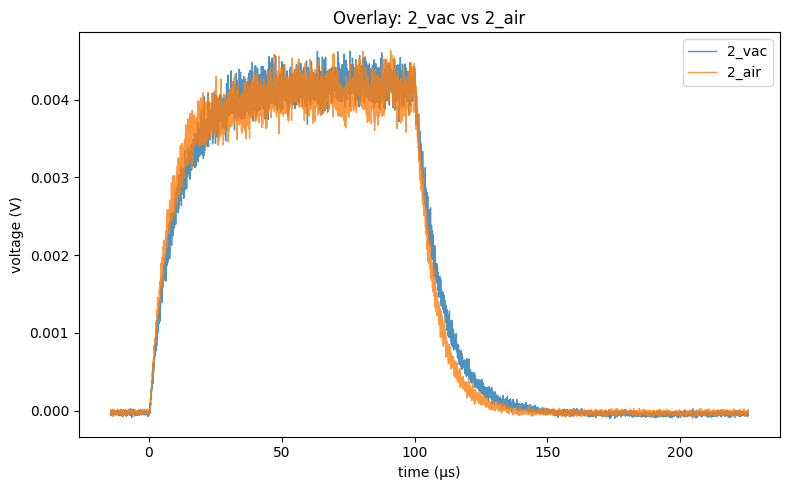
\includegraphics[width=1.0\linewidth]{../resources/figures/raw_overlay_2_vac_2_air.png}
  \caption{Overlay of a representative vacuum--air measurement pair (\texttt{2\_vac} and \texttt{2\_air}) after polarity correction.
  The plateau up to about \SI{100}{\micro\second} corresponds to the laser pulse duration.
  After the pulse ends, the transmitted intensity decays as the cavity empties, with a slightly faster decay for air due to additional intracavity losses.}
  \label{fig:raw_pair_overlay}
\end{figure}

Figure~\ref{fig:raw_pair_overlay} shows the raw traces of a vacuum--air pair after polarity correction.
At early times, the signal rises quickly and then remains at an approximately constant level for about \SI{100}{\micro\second}.
This plateau corresponds to the time interval during which the laser pulse injects light into the cavity and the intracavity intensity is sustained by the continuous input.

At $t\approx\SI{100}{\micro\second}$ the laser pulse ends, the cavity is no longer pumped, and the stored light decays due to cavity losses.
The subsequent decay is the ring-down signal of interest, from which the ring-down time constants $\tau_0$ (vacuum) and $\tau$ (air) will be extracted by fitting an exponential model as described in Sec.~\ref{sec:theory_crds}.
As expected, the decay in air is slightly faster than in vacuum, indicating an additional loss mechanism in the air-filled cavity that is attributed to molecular scattering.

\subsection{Selection of the fit window using a semilogarithmic plot}
\label{sec:evaluation_fit_window}

To extract $\tau$ reliably, the exponential decay must be fitted only in a time interval where a single-exponential behavior dominates and where the signal remains sufficiently above the noise floor.
A convenient diagnostic is a semilogarithmic representation: if the decay follows $V(t)\propto e^{-t/\tau}$, then $\ln V(t)$ should be approximately linear in time.
Figure~\ref{fig:semilog_exploratory} shows an exploratory semilog plot of the same vacuum--air pair for times beyond \SI{90}{\micro\second}.
A clear near-linear region is observed shortly after the end of the laser pulse, while at later times the scatter increases strongly and the semilog representation becomes dominated by noise.

Based on the exploratory semilog plots for all five measurement pairs, a common fit window was chosen as $t\in[\SI{102}{\micro\second},\,\SI{125}{\micro\second}]$.
The start time $t_\text{start}=\SI{102}{\micro\second}$ is chosen slightly after the nominal pulse end at \SI{100}{\micro\second} to avoid possible turn-off transients of the laser driver and detector response.
The end time $t_\text{end}=\SI{125}{\micro\second}$ is chosen conservatively to remain within the region that is still approximately linear on a semilog scale, before the signal approaches the noise floor.
This interval is comparatively short, which reduces the number of points contributing to the slope determination, but it avoids bias from noise-dominated late-time data and was found to be stable across all recorded traces.

\vspace{1em}
\begin{figure}[H]
  \centering
  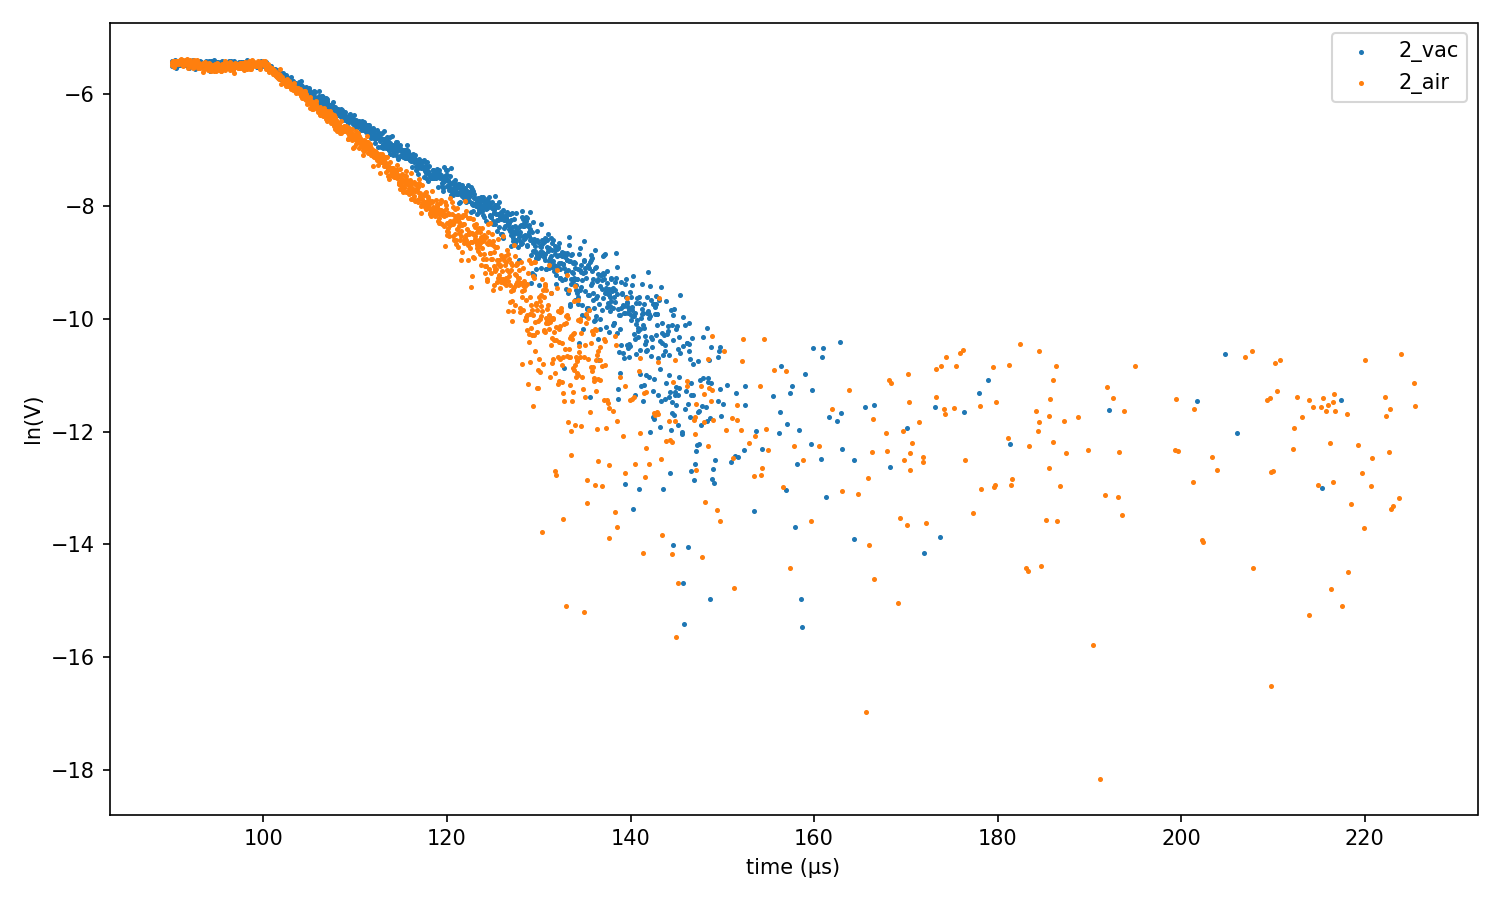
\includegraphics[width=1.0\linewidth]{../resources/figures/semilog_exploratory_2_vac_2_air.png}
  \caption{Exploratory semilog plot of the raw signal for the representative pair (\texttt{2\_vac} and \texttt{2\_air}).
  Shortly after the end of the laser pulse, the decay appears approximately linear in the semilogarithmic representation, consistent with a single-exponential ring-down.
  At later times the scatter increases strongly as the signal approaches the noise floor, motivating a restricted fit window.}
  \label{fig:semilog_exploratory}
\end{figure}

\subsection{Determination of the ring-down times by linear regression}
\label{sec:evaluation_fit_tau}

Within the selected fit window, the ring-down signal is modeled as a single exponential decay.
To account for the small baseline offset of the detector signal, a constant offset $C$ is estimated for each trace as the mean voltage in a late-time region where the ring-down has fully decayed and the signal is dominated by noise.
In practice, times $t\gtrsim\SI{160}{\micro\second}$ were found to be noise-dominated for all measurements, and this interval was therefore used consistently to compute $C$.
The baseline-corrected signal is then defined as $y(t)=V(t)-C$, where $V(t)$ denotes the recorded (polarity-corrected) photomultiplier voltage.
Assuming a single-exponential ring-down, one expects
\[
y(t)=A\,e^{-t/\tau}.
\]
Taking the natural logarithm yields the linear relation
\[
\ln y(t)=\ln A-\frac{t}{\tau}=a+b\,t,
\]
with intercept $a=\ln A$ and slope $b=-1/\tau$.
Thus, the desired ring-down time is obtained directly from the fitted slope as $\tau=-1/b$.

For each trace, the data points in the fit window $t\in[\SI{102}{\micro\second},\,\SI{125}{\micro\second}]$ were fitted with an ordinary least-squares (OLS) straight-line model.
Since no pointwise measurement uncertainties for the oscilloscope time axis and the photomultiplier voltage are available from the acquisition, the parameter uncertainties were estimated from the scatter of the data around the fitted line.
Concretely, the uncertainty of the slope $b$ was obtained from the covariance matrix returned by the OLS fit.
By error propagation, the corresponding uncertainty of the ring-down time is $\Delta\tau=\Delta b/b^{2}$.
Figure~\ref{fig:linreg_example} illustrates the linear regression for the representative pair \texttt{2\_vac} and \texttt{2\_air}.

\vspace{1em}
\begin{figure}[H]
  \centering
  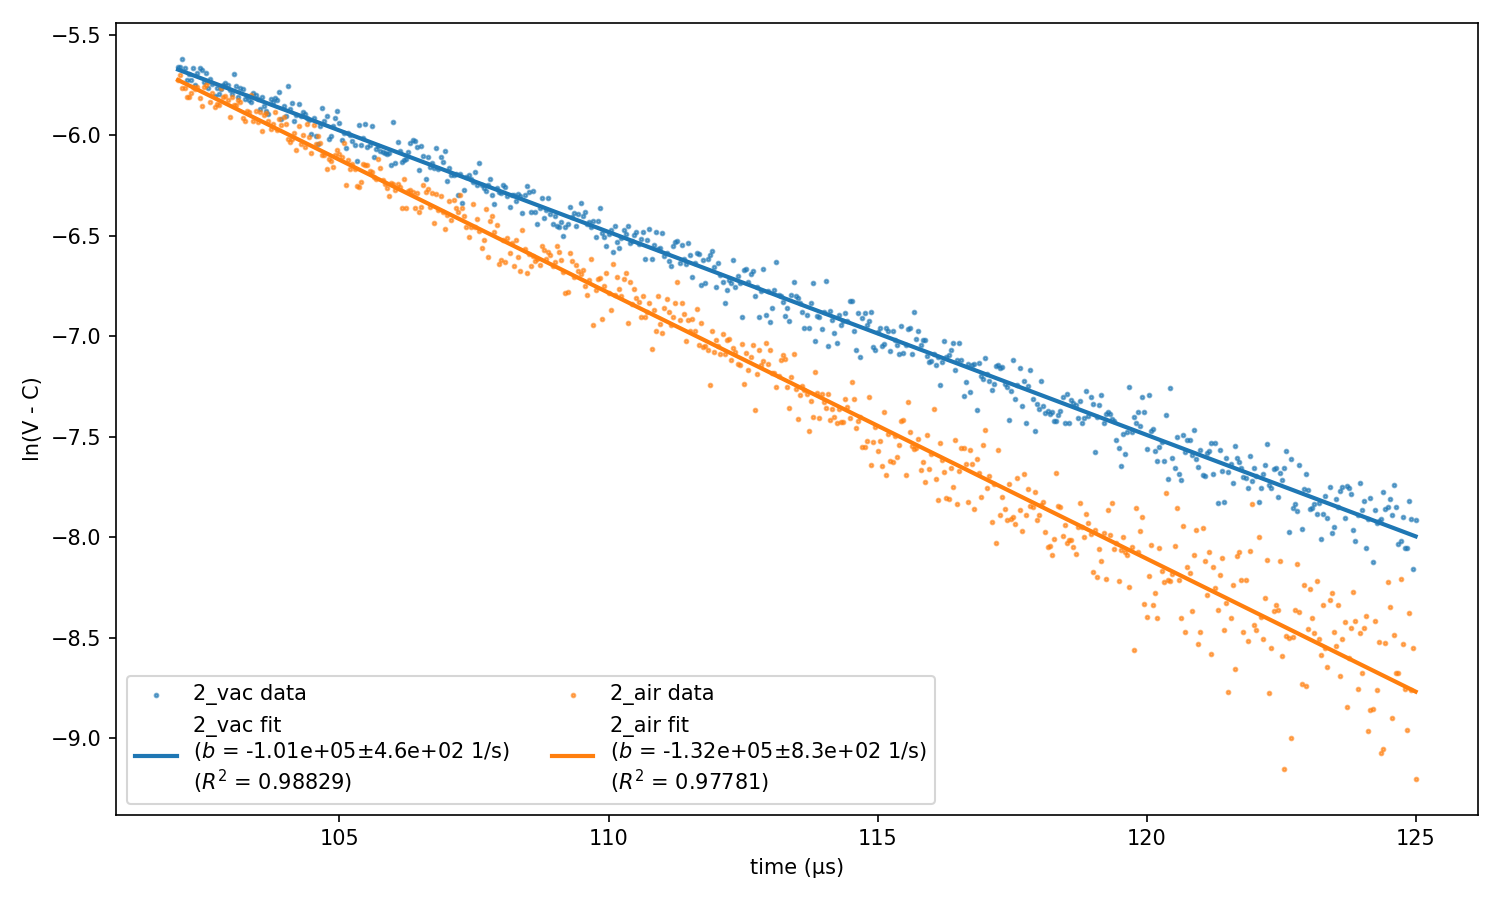
\includegraphics[width=1.0\linewidth]{../resources/figures/linreg_fit_2_vac_2_air.png}
  \caption{Linear regression of $\ln\!\bigl(y(t)\bigr)=\ln\!\bigl(V(t)-C\bigr)$ in the fit window $t\in[\SI{102}{\micro\second},\,\SI{125}{\micro\second}]$ for the representative pair \texttt{2\_vac} and \texttt{2\_air}.
  The fitted slopes $b$ (with uncertainties) correspond to the ring-down times via $\tau=-1/b$, and the steeper slope for air reflects the additional intracavity loss compared to vacuum.}
  \label{fig:linreg_example}
\end{figure}

The same analysis was applied to all ten traces, yielding five vacuum ring-down times $\tau_{0,i}$ and five air-filled ring-down times $\tau_i$.
The results are summarized in Table~\ref{tab:taus_all}.

\vspace{1em}
\begin{table}[H]
\centering
\caption{Ring-down times obtained from linear regression in the fit window $t\in[\SI{102}{\micro\second},\,\SI{125}{\micro\second}]$.
Vacuum measurements yield $\tau_{0,i}$ and air-filled measurements yield $\tau_i$, where $i=1,\dots,5$ denotes the measurement pair index.}
\label{tab:taus_all}
\begin{tabular}{c c c}
\toprule
Pair $i$ & $\tau_{0,i}$ (\si{\micro\second}) & $\tau_{i}$ (\si{\micro\second}) \\
\midrule
1 & $7.13 \pm 0.05$ & $6.57 \pm 0.05$ \\
2 & $9.90 \pm 0.04$ & $7.55 \pm 0.05$ \\
3 & $10.21 \pm 0.05$ & $8.40 \pm 0.05$ \\
4 & $9.19 \pm 0.05$ & $6.16 \pm 0.05$ \\
5 & $8.96 \pm 0.05$ & $8.91 \pm 0.05$ \\
\bottomrule
\end{tabular}
\end{table}

Table~\ref{tab:taus_all} shows that $\tau_{0,i}>\tau_i$ for all five pairs, as expected when additional intracavity losses are present in air.
However, the magnitude of the difference $\tau_{0,i}-\tau_i$ varies noticeably between pairs and is particularly small for pair~5.
Since the scattering coefficient is obtained from the difference of inverse ring-down times (Eq.~\eqref{eq:beta_from_taus}), such variations can have a strong impact on the extracted $\beta$ values.

\subsection{Experimental scattering coefficient}
\label{sec:evaluation_beta_exp}

From the measured ring-down times, the molecular scattering coefficient is obtained using Eq.~\eqref{eq:beta_from_taus}, with $c=\SI{2.99792458e8}{m/s}$ denoting the speed of light in vacuum.
For each vacuum--air measurement pair $i=1,\dots,5$, we compute
\[
\beta_i(\lambda)=\frac{1}{c}\left(\frac{1}{\tau_i}-\frac{1}{\tau_{0,i}}\right).
\]
The corresponding uncertainty is obtained by Gaussian error propagation, treating $\tau_{0,i}$ and $\tau_i$ as independent:
\[
\Delta\beta_i=\frac{1}{c}\sqrt{\left(\frac{\Delta\tau_i}{\tau_i^{2}}\right)^{2}+\left(\frac{\Delta\tau_{0,i}}{\tau_{0,i}^{2}}\right)^{2}}.
\]

The resulting values $\beta_i$ are summarized in Table~\ref{tab:beta_all}.

\vspace{1em}
\begin{table}[H]
\centering
\caption{Experimental scattering coefficients obtained from the five vacuum--air measurement pairs using Eq.~\eqref{eq:beta_from_taus}.}
\label{tab:beta_all}
\begin{tabular}{c c}
\toprule
Pair $i$ & $\beta_i$ (\si{m^{-1}}) \\
\midrule
1 & $(4.011 \pm 0.468)\times 10^{-5}$ \\
2 & $(10.458 \pm 0.317)\times 10^{-5}$ \\
3 & $(7.060 \pm 0.264)\times 10^{-5}$ \\
4 & $(17.826 \pm 0.442)\times 10^{-5}$ \\
5 & $(0.194 \pm 0.288)\times 10^{-5}$ \\
\bottomrule
\end{tabular}
\end{table}

\newpage
The values in Table~\ref{tab:beta_all} show a substantial spread between measurement pairs.
In particular, pair~5 yields a value consistent with zero within its uncertainty, which follows directly from the fact that $\tau_{0,5}$ and $\tau_{5}$ are nearly identical (Table~\ref{tab:taus_all}).
This highlights that the extracted scattering coefficient is highly sensitive to small differences between the vacuum and air ring-down times.

As a final experimental result, we report the mean scattering coefficient
\begin{equation}
\overline{\beta} = \frac{1}{5}\sum_{i=1}^{5}\beta_i = \boxed{\beta_{exp} = (7.910\pm 3.002)\times 10^{-5}\,\si{m^{-1}}} \, .
\label{eq:beta_exp}
\end{equation}
The uncertainty of $\overline{\beta}$ is taken as the standard error of the mean (SEM).
First, the scatter of the five individual values $\beta_i$ is quantified by the sample standard deviation $s_{\beta}$, which measures how strongly the $\beta_i$ vary from one measurement pair to the next.
If the five pairs are viewed as independent repeats of the same measurement, then averaging reduces purely statistical fluctuations.
The expected uncertainty of the mean value therefore decreases with the number of repeats and is given by
\[
\Delta\overline{\beta}=\mathrm{SEM}=\frac{s_{\beta}}{\sqrt{5}}.
\]

As a simple robustness check, we also evaluated the mean value excluding pair~5, because its $\beta_5$ value is consistent with zero within uncertainty.
This yields $\overline{\beta}_{(1\text{--}4)}=(9.839\pm 2.970)\times 10^{-5}\,\si{m^{-1}}$, i.e.\ an even larger deviation from the expected theoretical order of magnitude.
We therefore retain all five pairs in the final result and interpret the large run-to-run scatter as the dominant limitation of the measurement.

\subsection{Theoretical scattering coefficient}
\label{sec:evaluation_beta_theory}

To compare the experimental result with the theoretical Rayleigh prediction from Eq.~\eqref{eq:beta_rayleigh}, we evaluate $\beta(\lambda)$ under the ambient conditions during the measurements.
The ambient temperature and pressure were recorded once per vacuum--air pair and are listed in Table~\ref{tab:temp_pressure}.
Since the variations between pairs are small compared to the experimental scatter of $\beta_i$, the theoretical calculation is performed using the mean values $\overline{T}$ and $\overline{p}$.

\vspace{1em}
\begin{table}[H]
\centering
\caption{Ambient temperature and pressure recorded during the five vacuum--air measurement pairs.}
\label{tab:temp_pressure}
\begin{tabular}{c c c}
\toprule
Pair $i$ & $T_i$ (\si{\celsius}) & $p_i$ (\si{mbar}) \\
\midrule
1 & 19.7 & 1003.2 \\
2 & 20.1 & 1003.4 \\
3 & 20.2 & 1003.5 \\
4 & 20.4 & 1003.8 \\
5 & 20.4 & 1003.7 \\
\midrule
Mean & 20.16 & 1003.52 \\
\bottomrule
\end{tabular}
\end{table}

For the theoretical calculation we use
\[
\overline{T}=\SI{20.16}{\celsius}=\SI{293.31}{K},\qquad \overline{p}=\SI{1003.52}{mbar}=\SI{1.00352e5}{Pa}.
\]
The temperature was read from an analog glass thermometer with \SI{0.1}{\celsius} tick marks, so we take $\Delta T=\SI{0.1}{\celsius}$ as a reading uncertainty.
For the pressure, the manufacturer specifies an accuracy of $\Delta p=\SI{2.0}{mbar}$ (typ.\ at \SIrange{0}{50}{\celsius}), while the display digit of \SI{0.1}{mbar} is negligible on this scale~\cite{GPB3300Manual}.

The number density of air molecules is obtained from the ideal gas law in the form
\[
N=\frac{p}{k_B T},
\]
so that no explicit knowledge of the gas volume is required.
Here $k_B=\SI{1.380649e-23}{J/K}$ is the Boltzmann constant.
With Gaussian error propagation, the uncertainty of $N$ is
\[
\Delta N=\sqrt{\left(\frac{\partial N}{\partial p}\Delta p\right)^2+\left(\frac{\partial N}{\partial T}\Delta T\right)^2}
=\sqrt{\left(\frac{\Delta p}{k_B T}\right)^2+\left(\frac{p\,\Delta T}{k_B T^{2}}\right)^2}.
\]
Using $\overline{p}$ and $\overline{T}$ yields
\[
N=(2.4781\pm 0.0050)\times 10^{25}\,\si{m^{-3}}.
\]

For the Rayleigh calculation we take the laser wavelength as $\lambda=\SI{405}{nm}$ (manufacturer value, uncertainty not specified and therefore neglected).
The refractive index is taken from the literature table for standard air at \SI{0.400}{\micro\meter}, yielding $n=1.00028275$ (used as an approximation for \SI{405}{nm})~\cite{Miles2001}.
Inserting these values into Eq.~\eqref{eq:beta_rayleigh} gives
\begin{equation}
\boxed{\beta_\mathrm{th}=(3.967\pm 0.008)\times 10^{-5}\,\si{m^{-1}}} \, .
\label{eq:beta_th}
\end{equation}
Since $\beta_\mathrm{th}\propto 1/N$ for fixed $n$ and $\lambda$, the uncertainty is propagated as
\[
\frac{\Delta\beta_\mathrm{th}}{\beta_\mathrm{th}}=\frac{\Delta N}{N},
\qquad\Rightarrow\qquad
\Delta\beta_\mathrm{th}=\beta_\mathrm{th}\,\frac{\Delta N}{N}.
\]
The resulting $\Delta\beta_\mathrm{th}$ is very small compared to the experimental uncertainty of $\overline{\beta}$, so the theoretical uncertainty is negligible for the subsequent comparison.

% ------------------
% --- Discussion ---
% ------------------
\section{Discussion}
\label{sec:discussion}

The experimental result $\beta_\mathrm{exp}=(8\pm 3)\times 10^{-5}\,\si{m^{-1}}$ is larger than the theoretical prediction $\beta_\mathrm{th}=(3.967\pm 0.008)\times 10^{-5}\,\si{m^{-1}}$, and the dominant feature of the dataset is the large run-to-run scatter of the five pairwise values $\beta_i$ in Table~\ref{tab:beta_all}.
This scatter is much larger than the propagated uncertainties of individual fits, indicating that the overall measurement is not limited by the statistical precision of the linear regression but by systematic variations between measurement pairs.

A key point is that $\beta$ is extracted from a difference of decay rates, $\beta=\Delta(1/\tau)/c$.
As a consequence, small changes in the measured ring-down times $\tau$ and $\tau_0$ can lead to comparatively large changes in the inferred scattering coefficient.
A simple estimate illustrates this directly: for a typical pair, changing the air-filled ring-down time by only \SI{0.5}{\micro\second} changes $\beta$ by about $3.1\times 10^{-5}\,\si{m^{-1}}$, i.e.\ by an amount comparable to the expected Rayleigh signal itself.
This explains why the pairwise values $\beta_i$ can differ strongly even though each individual ring-down time is determined with an uncertainty of only about \SI{0.05}{\micro\second}.

The most plausible origin of such pair-to-pair variations is that the optical alignment of the cavity is not reproduced perfectly after refilling and re-optimizing.
Even small changes in the mirror angles can change how the light circulates inside the cavity and where it hits the mirror surfaces.
In some alignments the circulating beam remains well confined and losses are minimal, while in others a slightly larger fraction of light can be lost per round trip, for example by increased scattering on imperfect mirror regions or by small geometric losses (``clipping'') at edges or mounts.
Since the ring-down time $\tau$ is directly determined by these very small loss fractions, such alignment-dependent changes can noticeably shift $\tau$ and therefore strongly affect the extracted $\beta$.
The wooden laboratory table and the absence of a vibration-isolated optical table likely further increase sensitivity to small mechanical drifts, which can move the optimal alignment point on the time scale of repeated measurements.

In addition to alignment-related effects, residual scattering by remaining aerosols could provide a second possible contribution.
Although the incoming air is passed through a \SI{2}{\micro\meter} syringe filter, it cannot be ruled out that a small amount of particulate matter still enters the cavity.
Such particles would cause additional (non-molecular) light loss via scattering in the Mie regime, which would shorten the air-filled ring-down time and thus bias $\beta$ upward.
Whether this contribution changes significantly from one measurement to the next is difficult to judge from our data alone, but it is a plausible mechanism that could increase the measured loss in air compared to the pure Rayleigh expectation.

By contrast, uncertainties in the ambient pressure and temperature measurements have only a negligible effect on the theoretical prediction.
The propagated uncertainty of $\beta_\mathrm{th}$ from $\Delta p$ and $\Delta T$ is of order $10^{-7}\,\si{m^{-1}}$, which is far smaller than the experimental uncertainty of $\overline{\beta}$.
Similarly, the regression uncertainties of individual ring-down times are small compared to the observed scatter of the five $\beta_i$ values.
Therefore, improving the agreement between experiment and theory would primarily require improving the reproducibility of cavity conditions between vacuum and air measurements, for example by minimizing alignment changes between the two states, increasing mechanical stability, and reducing the influence of residual aerosols.

% ------------------
% --- Conclusion ---
% ------------------
\section{Conclusion}
\label{sec:conclusion}

In this experiment, Rayleigh scattering in air was studied as a weak but well-defined optical loss mechanism using cavity ring-down spectroscopy at $\lambda=\SI{405}{nm}$.
From five vacuum--air measurement pairs, the molecular scattering coefficient was determined to be $\beta_\mathrm{exp}=(8\pm 3)\times 10^{-5}\,\si{m^{-1}}$.
Using the recorded ambient pressure and temperature together with the Rayleigh prediction from Eq.~\eqref{eq:beta_rayleigh}, the theoretical expectation was found to be $\beta_\mathrm{th}=(3.967\pm 0.008)\times 10^{-5}\,\si{m^{-1}}$.

The analysis shows that the dominant limitation of the measurement is not the statistical uncertainty of the exponential fits, but the reproducibility of the cavity conditions between repeated measurements.
Since $\beta$ is obtained from a small difference of decay rates, small systematic changes in alignment between vacuum and air measurements can produce comparatively large variations in the extracted $\beta_i$ values and therefore dominate the overall uncertainty.
Further improvements would primarily require increased mechanical stability and a measurement procedure that minimizes alignment changes between the two cavity states, while keeping additional extinction contributions in air (e.g.\ due to residual aerosols) as small as possible.

% ----------------
% --- Appendix ---
% ----------------
\newpage
\section{Appendix}

Additional files:

\begin{itemize}
  \item \texttt{RAY\_Python.zip}
  \item \texttt{RAY\_LabReport.pdf}
\end{itemize}

% ------------------
% --- References ---
% ------------------
\setstretch{1.0}
\printbibliography[heading=bibintoc]

\section*{Author's Note}
AI-based writing and programming tools were used in a supporting role to refine the wording of this report and to assist in formatting Python and LaTeX code.
All research, scientific analysis, data evaluation, and interpretation were carried out independently by the authors.

% ------------------
% --- Lab Report ---
% ------------------
\newpage
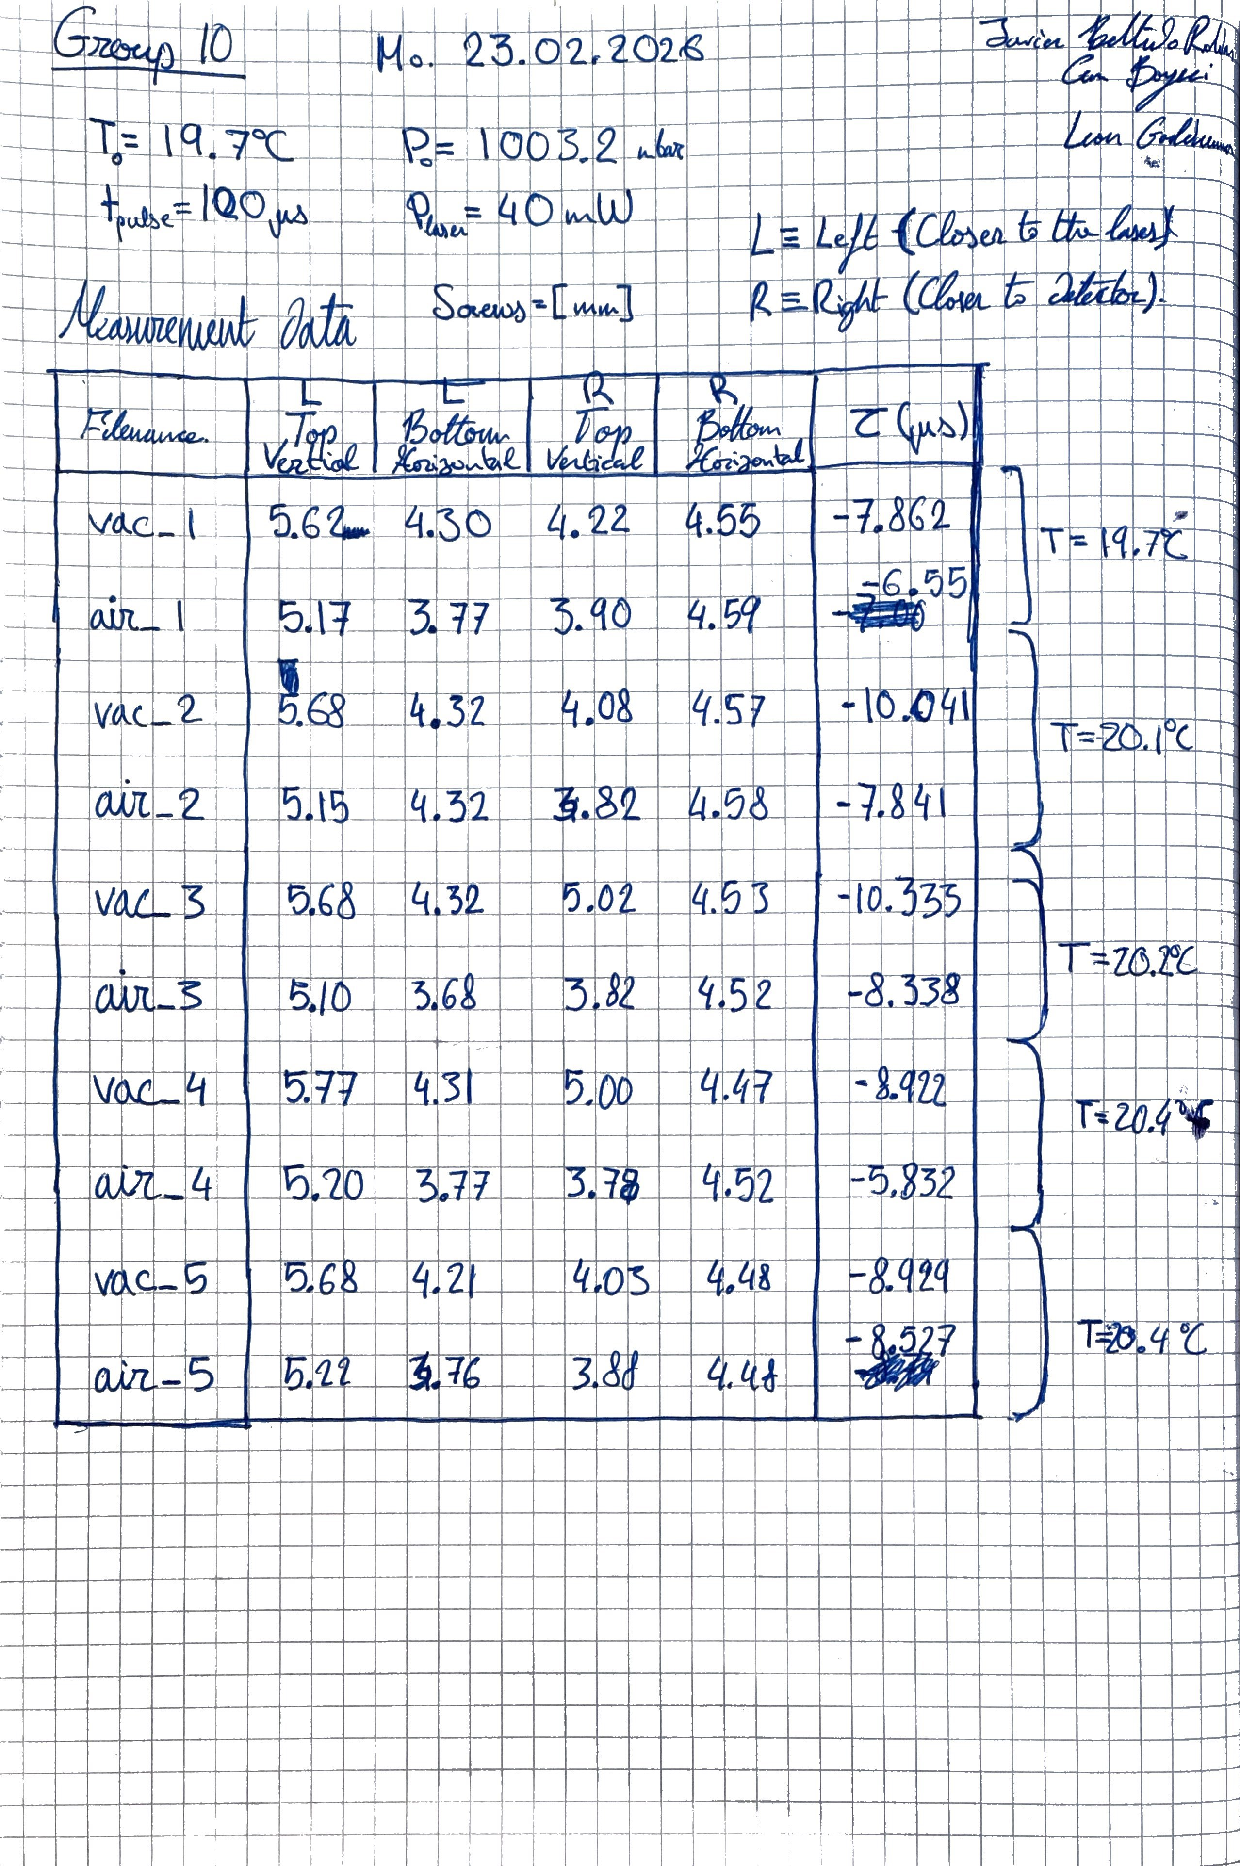
\includepdf[pages=-, scale=0.9, pagecommand={\thispagestyle{empty}}]{../resources/RAY_LabReport.pdf}

\end{document}
